\section{FOUR-SHIP TACTICS}

\subsection{OFFENSIVE TACTICS}

\subsection{DEFENSIVE TACTICS}

\begin{figure}[htbp]
    \centering
    \begin{tikzpicture}[figstyle]

        % coordinates
        \coordinate (lead_hot) at (0,0);
        \coordinate (wing_hot) at (-10,0);
        \coordinate (lead_cold) at ($(lead_hot) + (20,-40)$);
        \coordinate (wing_cold) at ($(wing_hot) + (20,-40)$);
        \coordinate (bandit) at (0,40);
        \coordinate (bandit_wing) at (-10,45);

        bandit wez
        \draw[fill=red!40] 
        (bandit_wing) -- ++(-60:15) arc (-60:-120:15) -- (bandit_wing);
        \draw[fill=red!40] 
        (bandit) -- ++(-60:15) arc (-60:-120:15) -- (bandit);

        % \draw[fill=color2!15] 
        % (lead_hot) -- ++(87:47) arc (87:93:47) -- (lead_hot);
        % \draw[fill=color2!15] 
        % (wing_hot) -- ++(87:52) arc (87:93:52) -- (wing_hot);

        % fighters
        \node[below] (lead_hot_fig) at (lead_hot) {
            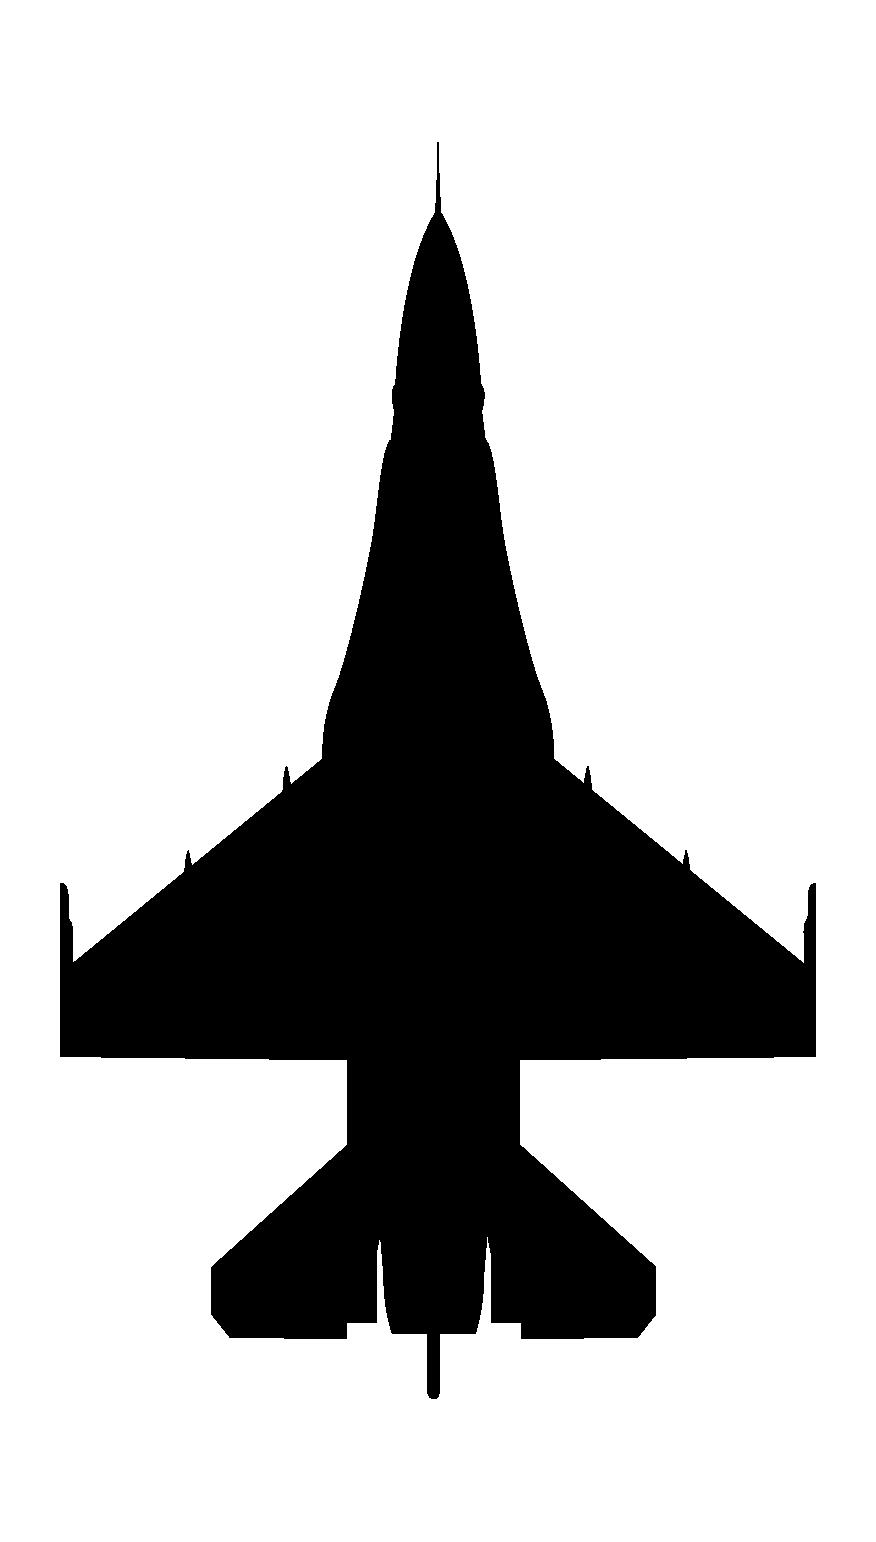
\includegraphics[
                width=7.5mm,
            ]{diagrams/aircraft/silhouette_f16_top.pdf}
        };
        \node[below] (wing_hot_fig) at (wing_hot) {
            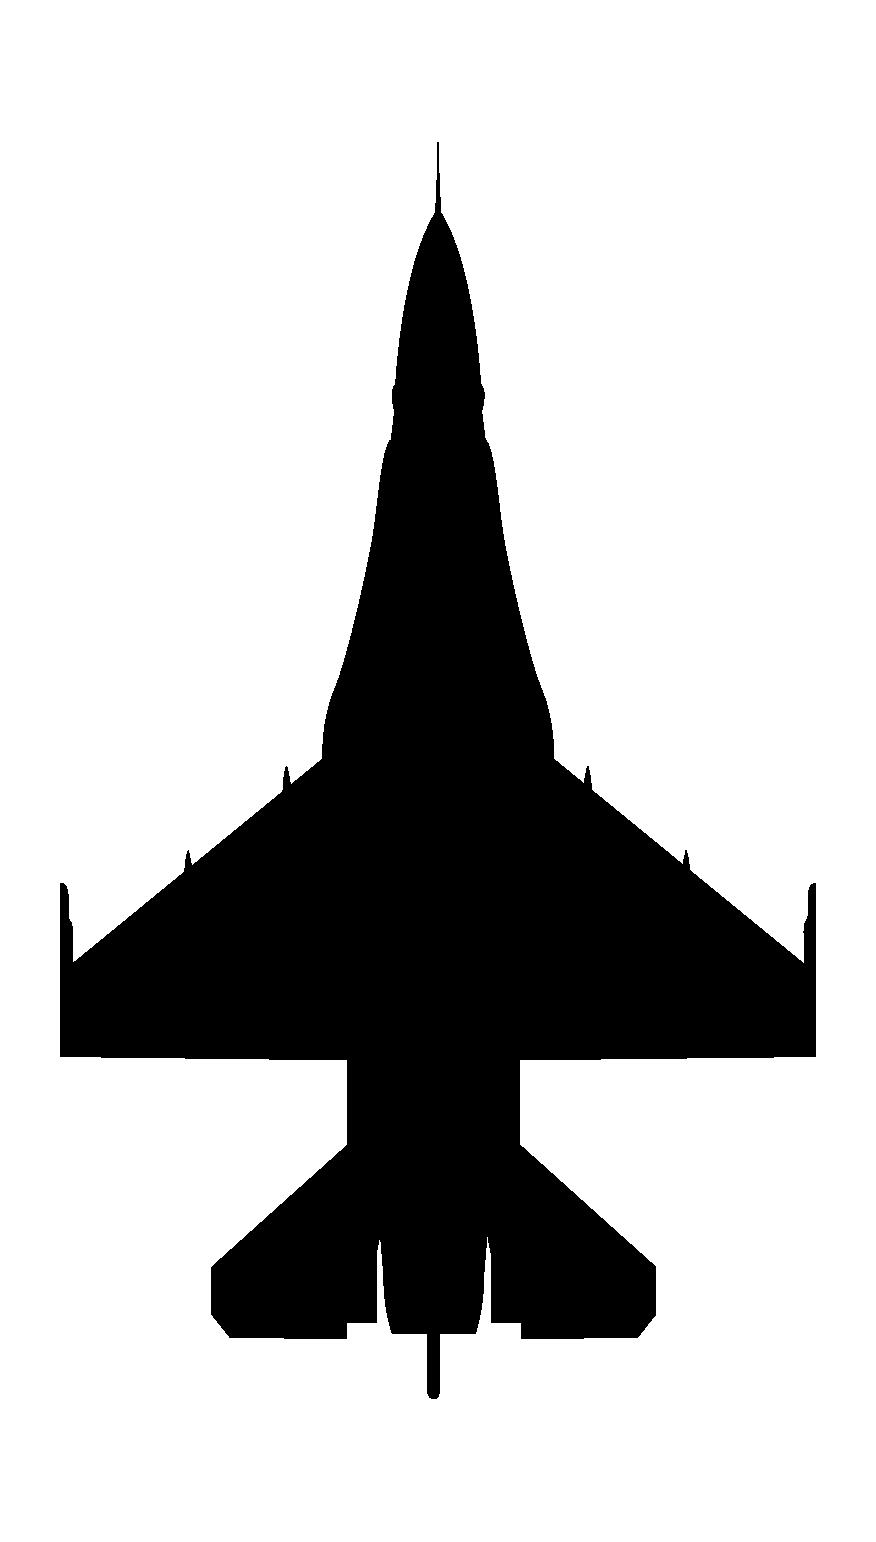
\includegraphics[
                width=7.5mm,
            ]{diagrams/aircraft/silhouette_f16_top.pdf}
        };
        \node[below, rotate=180] (lead_cold_fig) at (lead_cold) {
            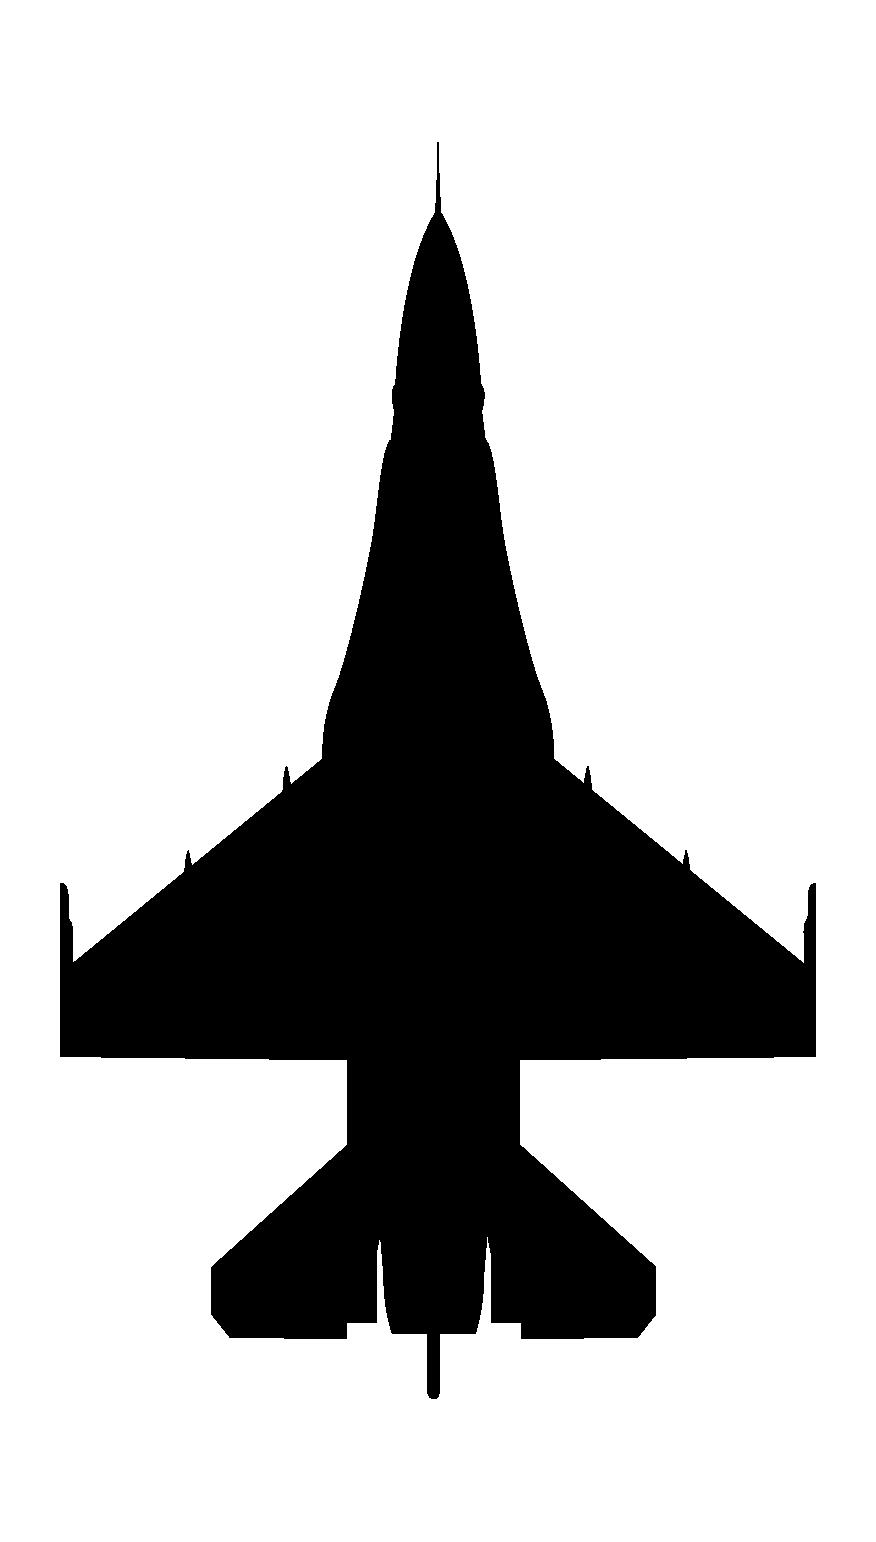
\includegraphics[
                width=7.5mm,
            ]{diagrams/aircraft/silhouette_f16_top.pdf}
        };
        \node[below, rotate=180] (wing_cold_fig) at (wing_cold) {
            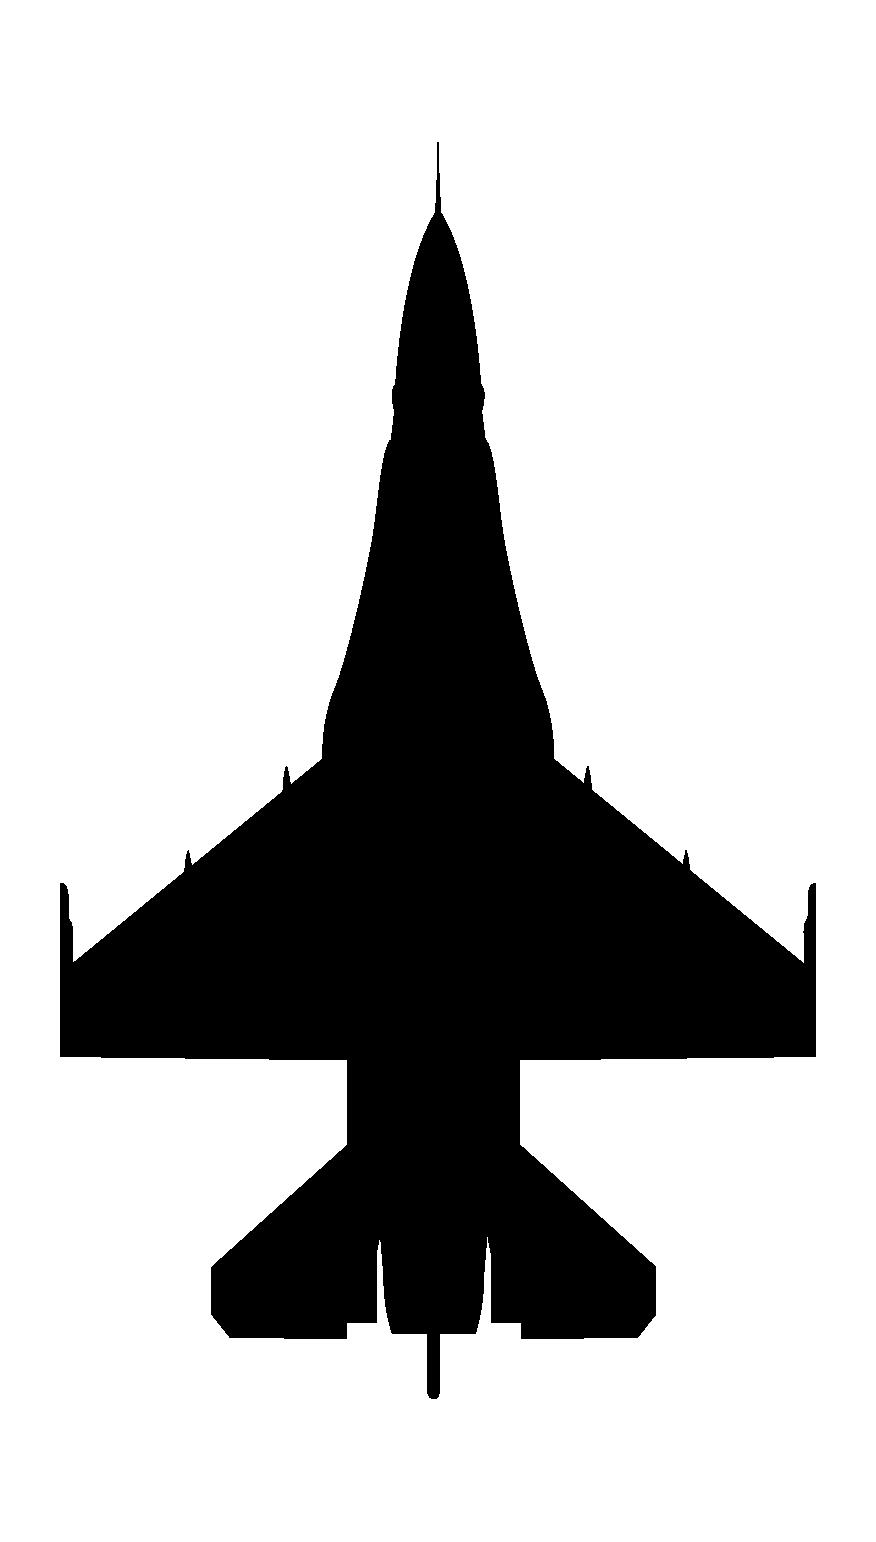
\includegraphics[
                width=7.5mm,
            ]{diagrams/aircraft/silhouette_f16_top.pdf}
        };
        
        % lead
        \draw[->] 
            (lead_hot) 
            -- ++(0,5)
            arc (180:0:10) 
            -- (lead_cold_fig.south);
        \draw[->] 
            (lead_cold) 
            -- ++(0,-5)
            arc (0:-180:10) 
            -- (lead_hot_fig.south);
        % wing
        \draw[->] 
            (wing_hot) 
            -- ++(0,5)
            arc (180:0:10) 
            -- (wing_cold_fig.south);
        \draw[->] 
            (wing_cold) 
            -- ++(0,-5)
            arc (0:-180:10) 
            -- (wing_hot_fig.south);

        % bandit
        \node[] (bandit_fig) at (bandit) {
            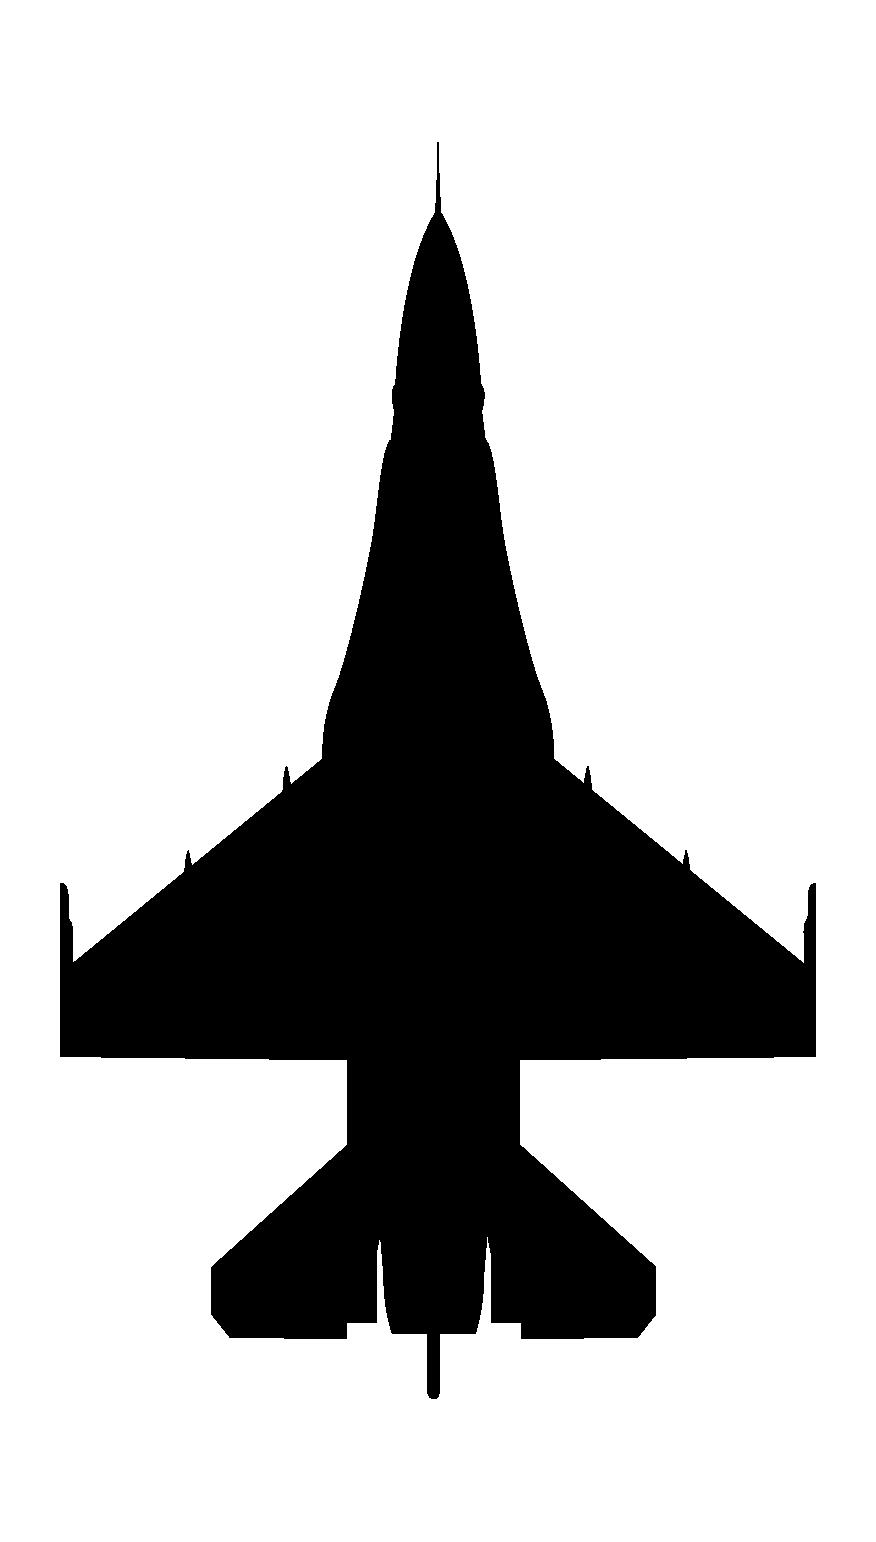
\includegraphics[
                    angle=180,
                    width=7.5mm,
            ]{diagrams/aircraft/silhouette_f16_top.pdf}
        };
        \node[] at (bandit_wing) {
            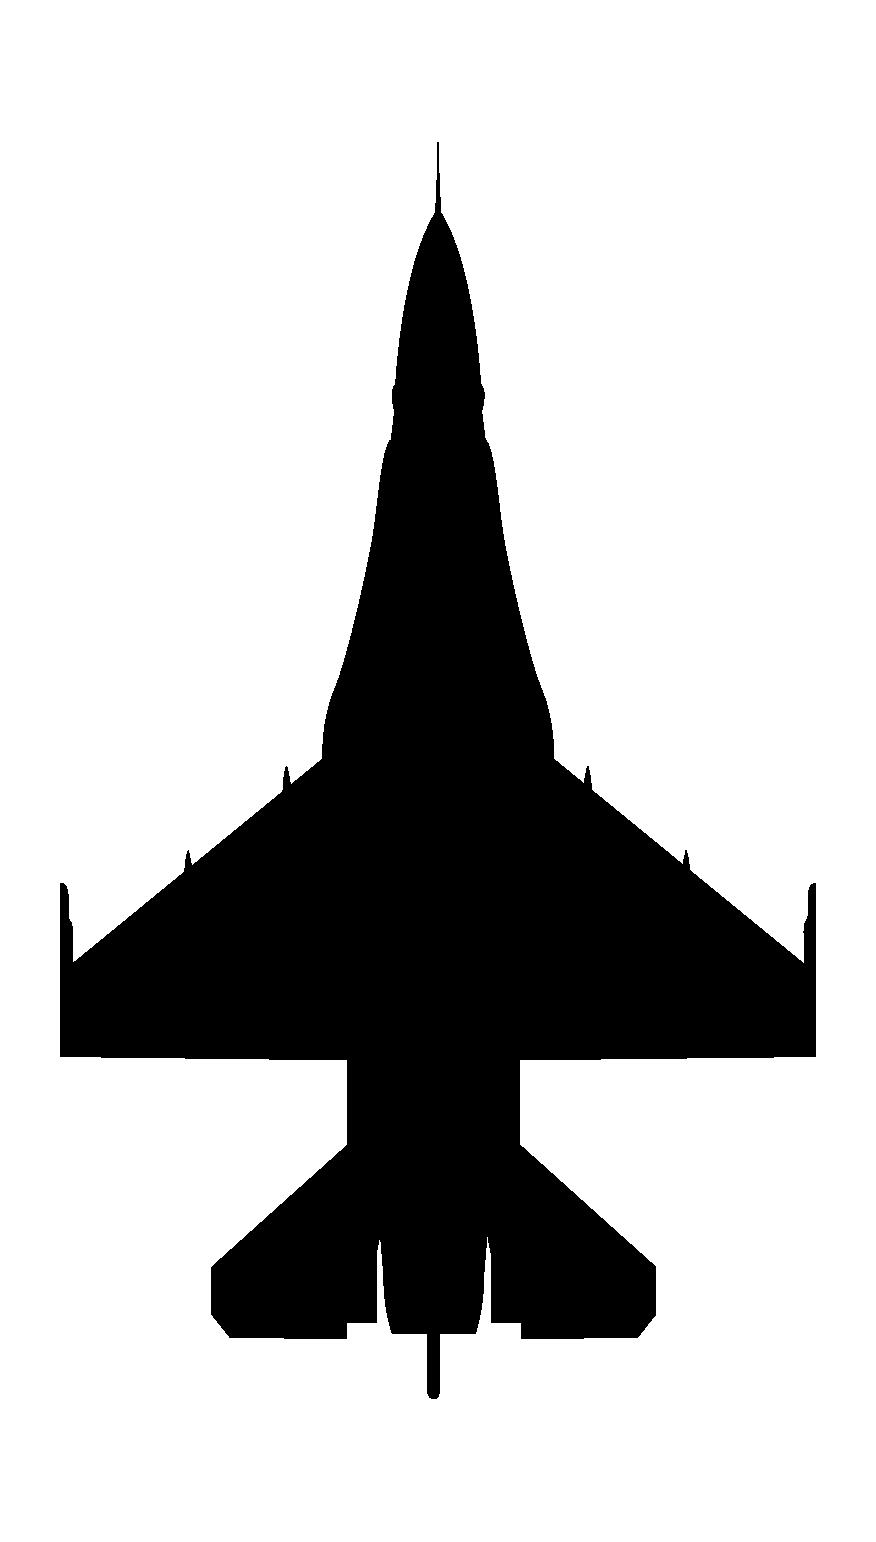
\includegraphics[
                    angle=180,
                    width=7.5mm,
            ]{diagrams/aircraft/silhouette_f16_top.pdf}
        };

        % labels
        \node[font=\small, align=right, left] at (wing_hot_fig.west) {Hot \\ Element};
        \node[font=\small, align=left, right] at (lead_cold_fig.west) {Cold \\ Element};
        \node[font=\small, right] at (bandit_fig.east) {Bandits};

    \end{tikzpicture}
    \caption{Four-ship grinder tactics}%
    \label{fig:ttp_aa:4ship:offensive:grinder}
\end{figure}